
\documentclass{article}
\usepackage{amsmath}
\usepackage[margin=1in]{geometry}
\usepackage{amsfonts}
\usepackage{hyperref}
\usepackage{graphicx}
\usepackage{siunitx}
\usepackage{cancel}
\usepackage{xfrac}


\begin{document}
	
	\title{Line Integrals}
	\author{Andy Chong Sam}
	\date{}
	\maketitle
	
	\section{Line Integral for Functions}
	
	\subsection{Overview}
	\par\noindent For a function, \(f(x,y)\) along a path \(S\), the most general form of a line integral is:
	
	\begin{flalign}
		\lim_{n \to \infty} f(x_i, y_i) \Delta S_i = \int_{C} f(x,y)\; dS
	\end{flalign}
	
	\begin{minipage}{.5\linewidth}		
		\par \noindent In Figure 1 we have a path \(S\) denoted by the red line. The path is divided into fairly large segments of length \(\Delta S\), but we can of course take infinitesimally small segments of length \(dS\).
	\end{minipage}
	\begin{minipage}[c]{.5\linewidth}
		
		\begin{center}
			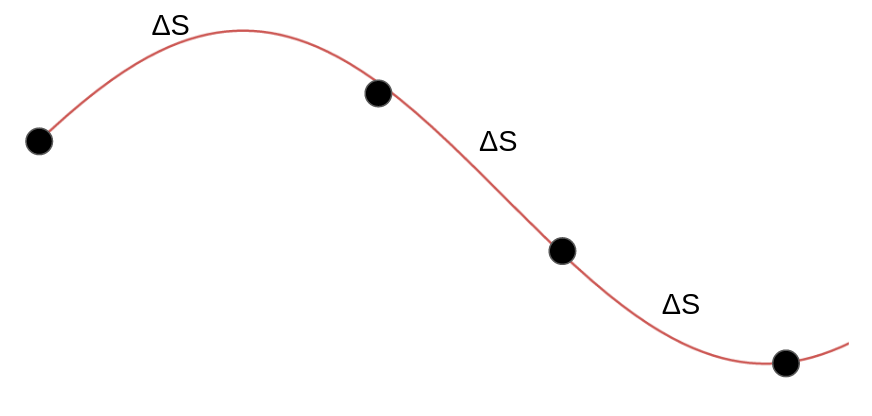
\includegraphics[width=5cm]{path.png}
		\end{center}
	
	\begin{center}
			Figure 1
	\end{center}
		
	\end{minipage}
	\newline
	\newline
	\par \noindent Not shown in Figure 1 is the function \(f\). We can imagine that \(f\) blankets the path traversed by \(S\). The line integral tells us the area underneath the path formed by \(S\).
	\newline
	\par \noindent If \(x\), and \(y\) can be described parametrically, then the line integral can be defined as:
	
	\begin{flalign}
		\int_{C} f(x,y)\; dS = \int_{C} f(x,y) \sqrt{x'(t)^2+ y'(t)^2}\; dt
	\end{flalign}
	\newpage
	\subsection{Derivation}
		\par \noindent We will derive Expression (2).
		
		\begin{minipage}{.5\linewidth}		
		\par \noindent In figure 2, we consider the path again, and we start by approximating the length through secant lines. We know that length of each secant line will be:
		
		\begin{flalign*}
			\overline{P_{i-1}P_i} = \sqrt{(x_i - x_{i-1})^2 + (y_i - y_{i-1})^2 }
		\end{flalign*}
	\end{minipage}
	\begin{minipage}[c]{.5\linewidth}
		
		\begin{center}
			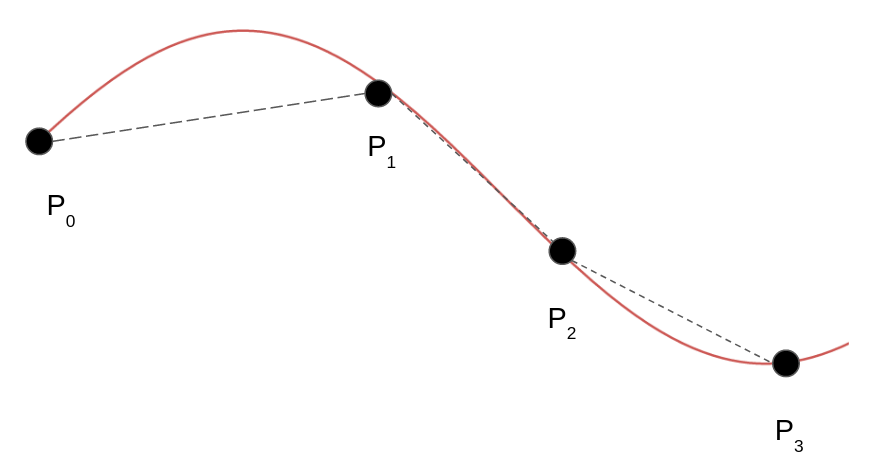
\includegraphics[width=5cm]{arc.png}
		\end{center}
		
		\begin{center}
			Figure 2
		\end{center}
		
	\end{minipage}
	\par \noindent If the curve is defined by a function \(f\), we know that through the mean value theorem there is a value \(c\) such that:
	\begin{flalign*}
		\frac{f(x_i) - f(x_{i-1})}{x_{i} - x_{i-1}} = f'(c) \\
		f(x_i) - f(x_{i-1}) = f'(c)(x_{i} - x_{i-1})
	\end{flalign*}

	\par\noindent Let's say that \(x_{i} - x_{i-1} = \Delta x\). If \(y=f(x)\), then \(y_{i} - y_{i-1} = f'(c)(x_{i} - x_{i-1})\). We can now rewrite the secant line:
	
	\begin{flalign*}
		\overline{P_{i-1}P_i} = \sqrt{ \Delta x^2 + (f'(c)\Delta x)^2} \\
		= \Delta x \sqrt{1 + f'(c)^2}
	\end{flalign*}
		
	\par \noindent The estimated length of the entire curve is therefore:
	
	\begin{flalign*}
		L = \sum_{i=1}^{n}\; \overline{P_{i-1}P_i} = \sum_{i=1}^{n}\;\Delta x \sqrt{1 + f'(c)^2}
	\end{flalign*}
	
		\par \noindent If we draw more secant lines, with smaller lengths for \(\overline{P_{i-1}P_i}\) we will improve the length estimate. If we take infinitesimally small segments we get an integral. This expression gives us the length of a curve:
	
		\begin{flalign*}
		L = \lim_{n \to \infty} \sum_{i=1}^{n}\;\Delta x \sqrt{1 + f'(c)^2}
	\end{flalign*}
	
	
	\begin{flalign}
		L = \int_{a}^{b} \sqrt{1 + f'(x)^2}\; dx
	\end{flalign}
	
	\par\noindent Now let's suppose that the path is not a function where \(y\) depends on \(x\) but is instead one in which \(x\) and \(y\) are represented parametrically, depending on t. 
	\newline
	\par\noindent One way to visualize this is to imagine that you are a satellite viewing straight down at a specific location. The land, hills, rivers, valleys, and other features are defined by \(f\), but for whatever reason we are only interested in a specific path \(S\) on this terrain. If \(S\) crosses a hill at \(t=1\), we expect this point to have its own \(x\) and \(y\) values. If at  \(t=5\) it passes over a plain, we would expect that area to have a lower \(y\) value than when it passed the hill. The line integral gives us the area underneath this path.
	\newline
	\par \noindent To complete the integration, we restate Expression (3) in terms of \(t\), so if \(f(x,y)=(\;x(t), y(t)\;)\), through implicit differentiation we get:
	
	\begin{flalign*}
	L = \int_{a}^{b} \sqrt{1 + f'(x)^2}\; dx = \int_{a}^{b} \sqrt{1 + (\frac{\sfrac{dy}{dt}}{\sfrac{dx}{dt}})^2}\; \frac{dx}{dt} dx \\
	= \int_{a}^{b} \sqrt{(\frac{\sfrac{dx}{dt}}{\sfrac{dx}{dt}})^2 + (\frac{\sfrac{dy}{dt}}{\sfrac{dx}{dt}})^2}\; \frac{dx}{dt} dx \\
	= \int_{a}^{b} \frac{1}{\sfrac{dx}{dt}} \sqrt{ (\frac{dx}{dt})^2 + (\frac{dy}{dt})^2} \frac{dx}{dt} dt \\
	= \int_{a}^{b} \sqrt{ (\frac{dx}{dt})^2 + (\frac{dy}{dt})^2} \; dt 
	\end{flalign*}
	
	\par\noindent The last step is to take into account the value of function \(f\) (in our analogy, the area underneath a segment of S will be different if we're looking at a hill vs a plain). We are left with expression 2:
	
	 \begin{flalign*}
	 \int_{C} f(x,y)\;dS =	\int_{a}^{b} f(x,y) \sqrt{ (\frac{dx}{dt})^2 + (\frac{dy}{dt})^2} \; dt = \int_{C} f(x,y) \sqrt{x'(t)^2+ y'(t)^2}\; dt
	 \end{flalign*}
 
 	 \subsection{Examples}
 	 
 	 \framebox{
 	 	\parbox{\linewidth}{
 	 		\par\noindent \textbf{Ex. 1} Evaluate \(\int_{C}6x\;dS\) where C is \(y=x^2\), where \(x(t)=t\) and \(y(t)=t^2\) and \(-1 \leq t \leq 2\).
 	 		\newline
 	 		\par\noindent Source: Paul's Online Notes 
 	 		\par\noindent \text{https://tutorial.math.lamar.edu/Problems/CalcIII/LineIntegralsPtI.aspx}
 	 		\newline
 	 		\begin{flalign*}
 	 			x'(t) = 1 \;\; y'(t) = 2t \\
 	 			\text{Because \(x=t\), } 6x = 6t
 	 		\end{flalign*}
  		
  			\par\noindent So this is the integral we want to evaluate:
  			
  			\begin{flalign*}
  				\int_{-1}^{2}6t\sqrt{1+(2t)^2}\;dt
  			\end{flalign*}
  		
  			\par\noindent We'll do a u-substitution with \(u= 1+4t^2 \):
  			
  			\begin{flalign*}
  				\int_{-1}^{2}6t\sqrt{1+(2t)^2}\;dt = 6\frac{(1+4t^2)^{\frac{3}{2}}}{12} \Big|_{-1}^{2}  = \frac{17^{\frac{3}{2}} - 5^{\frac{3}{2}}}{12}
  			\end{flalign*} 		
 	 }}
 	\newline
 	\newline
 	\newline
  	 \framebox{
 	\parbox{\linewidth}{
 		 \par\noindent \textbf{Ex. 2} Evaluate \(\int_{C}x^2 + y^2\;dS\), where C is the line segment that runs from \((0,0)\) to \((1,1)\)
 		 	\newline
 		 \par\noindent Source: Larson, Calculus 6th Edition, pg 1061
 		 \newline
 		 \par\noindent We can easily parameterize a line segment with the following formula:
 		 \begin{flalign*}
 		 	x(t) = x_1(1-t) + x_2(t) \\
 		 	y(t) = y_1(1-t) + y_2(t) \\
 		 \end{flalign*}
 	 	\par\noindent This gets us:
 	 	\begin{flalign*}
 	 		 x(t) = (0)(1-t) + (1)(t) = t\\
 	 		y(t) = (0)(1-t) + (1)(t) = t \\
 	 	\end{flalign*}
  		\par\noindent We observe that \(x'(t) = y'(t) = 1\). Since \(x(t)=y(t)=t\), \(f\) can be rewritten as \(2t^2\). We can now work on the integral:
  		\begin{flalign*}
  			\int_{0}^{1} 2t^2 \sqrt{2}\;dt = 2\sqrt{2}\;\frac{t^3}{3}\Big|_{0}^{1} = \frac{2}{3}\sqrt{2} 
  		\end{flalign*}
 
 		 
 }}
 	\newline
\newline
\newline
\framebox{
	\parbox{\linewidth}{
	\par\noindent \textbf{Ex. 3} Evaluate \(\int_{C}x^2 + y^2 + z^2\;dS\), where C is defined by \(x(t)=\sin t\),\(y(t)=\cos t\), and \(z=2\), \(0 \leq t \leq \frac{\pi}{2}\).
	\newline	
	\par\noindent Source: Larson, Calculus 6th Edition, pg 1061
	\newline
	\begin{flalign*}
		x'(t) = \cos t \;\;\;\; y'(t) = -\sin t \;\;\;\;  z'(t) = 0
	\end{flalign*}

	\par\noindent Restating \(f\) in terms of t we get:
	
	\begin{flalign*}
		x^2 + y^2 + z^2 = \sin^2 t + cos^2 t + 4 = 5
	\end{flalign*}

	\par\noindent We can now evaluate the integral:
	
	\begin{flalign*}
		\int_{0}^{\frac{\pi}{2}}5\sqrt{\cos^2 t + \sin^2 t }\;dt = \int_{0}^{\frac{\pi}{2}}5\;dt = 5t \Big|_{0}^{\frac{\pi}{2}} = \frac{5\pi}{2}
	\end{flalign*}
}}
 	\newline
\newline
\newline
\framebox{
	\parbox{\linewidth}{
	\par\noindent \textbf{Ex. 4} Evaluate \(\int_{C}xy\;dS\), C is defined by \(x(t)=4t\) and \(y(t)=3t\), \(0 \leq t \leq 1\).
	\newline
	\par\noindent Source: Larson, Calculus 6th Edition, pg 1061
	\newline
	\begin{flalign*}
		x'(t) = 4 \;\;\; y'(t) = 3
	\end{flalign*}
	\par\noindent We can restate \(f\) in terms of t:
	\begin{flalign*}
		xy = (4t)(3t) = 12t^2
	\end{flalign*}
	\par\noindent The integral can now be setup:
	\begin{flalign*}
		\int_{0}^{1}12t^2(5)\;dt = 20t^3  \Big|_{0}^{1} = 20
	\end{flalign*}
	
}}
 	\newline
\newline
\newline
\framebox{
	\parbox{\linewidth}{
		\par\noindent \textbf{Ex. 5} Evaluate \(\int_{C}xy^4\;dS\) where C is defined as the right half of the circle defined by \(x^2 + y^2 = 16\).
		\newline
		\par\noindent Source: Stewart, Calculus 8th Edition pg 1084
		\newline
		\par\noindent Since we are dealing with the right half of the circle, \(-\frac{\pi}{2} \leq t \leq \frac{\pi}{2}\).
		
		\begin{flalign*}
x(t) = 4\cos t \;\;\; x'(t) = -4\sin t \\
y(t)= 4\sin t \;\;\; y'(t)=4\cos t
		\end{flalign*}
	
		\par\noindent Let's redefine \(f\) in terms of \(t\):
		
		\begin{flalign*}
			xy^4 = (4\cos t)(4 \sin t)^4
		\end{flalign*}
	
		\par\noindent The full integral to evaluate is now:
		
		\begin{flalign*}
			\int_{-\frac{\pi}{2}}^{\frac{\pi}{2}} (4\cos t)(4 \sin t)^4 \sqrt{16\sin^2t + 16\cos^2t}\;dt
		\end{flalign*}
	
		\par\noindent This is a good candidate for integration by parts. We'll pick \(u=\sqrt{16sin^2t + 16cos^2t}\) 
		\par\noindent and \(v'=(4\cos t)(4\sin t)^4\). Let's figure out \(u'\):
		\begin{flalign*}
			u=\sqrt{16\sin^2t + 16\cos^2t} = \sqrt{16(\sin^2t + \cos^2t)} = \sqrt{16}\;\;\;\text{So \(u' = 0\)} 
		\end{flalign*}
	
		\par\noindent Let's determine \(v\) from \(v'\):
		
		\begin{flalign*}
			\int (4\cos t)(4 \sin t)^4\;dt = \frac{1024}{5} \sin^5t + C
		\end{flalign*}
	
		\par\noindent We can now assemble the final integral. Since \(u'\) is 0, we only need to integrate \(uv\):
		
		\begin{flalign*}
\int_{-\frac{\pi}{2}}^{\frac{\pi}{2}} (4\cos t)(4 \sin t)^4 \sqrt{16\sin^2t + 16\cos^2t}\;dt = \frac{1024\sqrt{16}}{5}\sin^5t  \Big|_{-\frac{\pi}{2}}^{\frac{\pi}{2}} = \frac{2048\sqrt{16}}{5}
		\end{flalign*}
	
		
		
}}
	\section{Line Integral for Vector Fields}
	
	\par\noindent Here are three equivalent definitions of the line integral for vector fields:
	
	\begin{flalign}
		 \int_{C} \vec F \cdot \vec T\;dS = \int_{C} F(\;r(t)\;)\;r'(t)\; dt = \int_{C} \vec F \;dR
	\end{flalign}

	\par\noindent To assist with seeing the intuition of Expression (4) we start with the left-most definition and Figure 3. The dotted black lines represent a vector field \(\vec F\). We want to study the effect of \(\vec F\) on a particle, the black circle, along path \(S\). We will define \(S\) with a vector function \(r(t)\).

	\begin{center}
		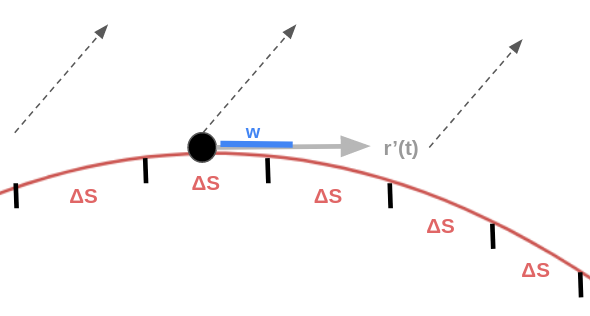
\includegraphics[width=10cm]{vecline.png}
	\end{center}

\begin{center}
	Figure 3
\end{center}

\par\noindent To understand the effect of \(\vec F\) on the particle, we also need to consider the tangent vector \(r'(t)\), and the projection of \(\vec F\) onto \(r'(t)\). In Figure 3, this is denoted by \(w\), and we can calculate it with a dot product and the magnitude of the tangent vector:

\begin{flalign*}
	w = \frac{ \vec F \cdot r'(t)}{||\;r'(t)\;||}
\end{flalign*}

\par\noindent Symbolically, we refer to the projection as the dot product of  \(\vec F\) and \(\vec T\), where \(\vec T = \frac{r'(t)}{||\;r'(t)\;||}\).
\newline
\par\noindent In Figure 3, the curve is arbitrarily subdivided into chunks of \(\Delta S\). We can now imagine infinitesimally small segments of \(dS\) instead. From Expression (2) we know that \(dS=\sqrt{x'(t)^2 + y'(t)^2}\;dt\). If \(r(t)\) is a vector function describing \(S\) made up of \(x\) and \(y\), then \(dS\) is nothing more than the magnitude \(r'(t)\) along with \(dt\):

\begin{flalign*}
	dS =\sqrt{x'(t)^2 + y'(t)^2}\;dt = ||\;r'(t)\;||\;dt
\end{flalign*}
\par\noindent We've now derived the practical form for the line integral of vector fields:

\begin{flalign*}
	\int_{C} F \cdot T\;dS = \int_{C} F(\;r(t)\;)\;r'(t)\; dt
\end{flalign*}
\par\noindent The expression \(r'(t)dt\) is sometimes stated as \(dS\), which gets us the right most equation of Expression (4):

\begin{flalign*}
	\int_{C} F(\;r(t)\;)\;r'(t)\; dt = \int_{C} \vec F \;dR
\end{flalign*}
\newpage
\framebox{
	\parbox{\linewidth}{
	\par\noindent \textbf{Ex. 6} Evaluate \(\int_{C} \vec F dR\) where \(\vec F = xy\; \vec i + xz\;\vec j + yz\;\vec k\) and the path C is defined by \(t \; \vec i + t^2\;\vec j + 2t \;\vec k\). 
	\newline
	\par\noindent Source: Larson, Calculus 6th Edition, pg 1062
	\newline
	\par\noindent We first define \(F\) in terms of \(t\) using \(r(t)\):
	
	\begin{flalign*}
		<xy, yz, yz> = <(t)(t^2), (t)(2t), (t^2)(2t) > = <t^3, 2t^2, 2t^3> 	
	\end{flalign*}

	\par\noindent Next we evaluate \(r'(t)\):
	
	\begin{flalign*}
		r'(t) = <1,2t,2>
	\end{flalign*}

	\par\noindent Assemble and evaluate the integral:
	
	\begin{flalign*}
		\int_{0}^{1} <t^3, 2t^2, 2t^3> \cdot <1,2t,2> \;dt \\
		\int_{0}^{1} 9t^3 dt = \frac{9}{4}t^4 \Big|_{0}^{1} = \frac{9}{4}
	\end{flalign*}
}}
\newline
\newline
\newline

\framebox{
	\parbox{\linewidth}{
	\par\noindent\textbf{Ex. 7} Evaluate \(\int_{C} \vec F dR\)  where \(\vec F = xy^2\;\vec i -x^2\;\vec j\) and C is defined by \(t^3\; \vec i + t^2\; \vec j\), where \(0 \leq t \leq 1\).	
	\newline
	\par\noindent Source: Stewart, Calculus 8th Edition pg 1085
	\newline
	
	\par\noindent We first define \(F\) in terms of \(t\) using \(r(t)\):
	
	\begin{flalign*}
		<xy, yz> = <t^7, -t^6>
	\end{flalign*}

	\par\noindent Evaluate \(r'(t):\)
	
	\begin{flalign*}
		r'(t) = <3t^2, 2t>
	\end{flalign*}

	\par\noindent Evaluate the integral:
	
	\begin{flalign*}
		\int_{0}^{1} <t^7, -t^6> \cdot <3t^2, 2t> \; dt \\
		\int_{0}^{1} 3t^9 - 2t^7 \; dt = (\frac{3}{10}t^{10} - \frac{1}{4}t^8)\Big|_{0}^{1} = \frac{1}{20}
	\end{flalign*}	
}}

\end{document}